\section{Overview}
An operating system is a huge and complex program that 
administrates the hardware of a computer (in this case the
STK1000 microcontroller) and offers all the different devices
to the programmer through a nice and relatively easy interface.
This makes it possible for the programmer to write rich
programs without having to think too much about task management,
permissions to different users and how to control and handle
the hardware, which is just a few important features of an
operating system.\\
\\
In order for an operating system, like Linux, 
to work with all the different hardware out there, it will need
device drivers for the different devices. These drivers is a 
special kind of software that runs \textit{between} the operating
system and the hardware and makes it possible
for the operating system to use the specific device.
\begin{figure}[h]
  \centerline{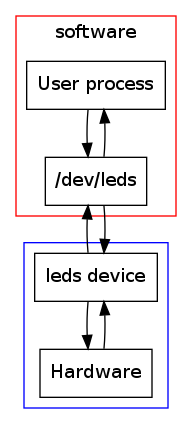
\includegraphics[width=100px]{graphics/device_driver.png}}
  \caption{The location of a device driver in the Linux environment}
  \label{device-driver}
\end{figure}
This could
not have been done if it had not been for a common interface that 
the different drivers could implement. Linux offers such an 
interface, and it is described in the book 
Linux Device Drivers \cite{linux-device-drivers}.\\
\\
